\usecasebase{Visualizzazione messaggio di selezione di una pietanza con allergene}
\label{usecase:Visualizzazione messaggio di selezione di una pietanza con allergene}

\begin{figure}[h]
	\centering
	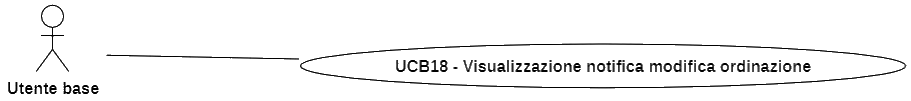
\includegraphics[width=0.9\textwidth]{./uml/UCB18.png} 
	\caption{Visualizzazione messaggio di selezione di una pietanza con allergene}
	\label{fig:UCB20}
  \end{figure}

\begin{itemize}
	\item \textbf{Attore principale:} Utente base.

	\item \textbf{Precondizione:}
	      L'Utente base ha selezionato una pietanza che contiene un allergene di cui lui è intollerante (vedi \autoref{usecase:Seleziona pietanza}).

	\item \textbf{Postcondizione:}
	      L'Utente base visualizza il messaggio che lo avverte che ha selezionato una pietanza che contiene un allergene di cui lui è intollerante.

	\item \textbf{Scenario principale:}
	      \begin{enumerate}
		      \item Il Sistema riconosce che la pietanza selezionata dall'Utente base contiene un allergene di cui lui è intollerante;
		      \item Il Sistema mostra un messaggio che avverte l'Utente base che ha selezionato una pietanza che contiene un allergene di cui lui è intollerante;
		      \item L'Utente base visualizza il messaggio.
	      \end{enumerate}
\end{itemize}
